\documentclass{article}
\usepackage[spanish]{babel}
\usepackage{graphicx} % Required for inserting images
\usepackage{lipsum}
\usepackage[a4paper, total={6in, 8in}]{geometry}
\usepackage{setspace}
\usepackage[utf8]{inputenc}
\usepackage{csquotes}
\usepackage{amssymb,amsmath,amsthm, amsfonts}

\usepackage{hyperref}
\hypersetup{
    colorlinks=true,
    linkcolor=blue,
    filecolor=magenta,      
    urlcolor=cyan,
    pdftitle={Overleaf Example},
    pdfpagemode=FullScreen,
    }
\urlstyle{same}

\usepackage{xcolor}
\usepackage{listings}

\definecolor{mGreen}{rgb}{0,0.6,0}
\definecolor{mGray}{rgb}{0.5,0.5,0.5}
\definecolor{mPurple}{rgb}{0.58,0,0.82}
\definecolor{backgroundColour}{rgb}{0.95,0.95,0.92}

\lstdefinestyle{CStyle}{
    backgroundcolor=\color{backgroundColour},   
    commentstyle=\color{mGreen},
    keywordstyle=\color{magenta},
    numberstyle=\tiny\color{mGray},
    stringstyle=\color{mPurple},
    basicstyle=\footnotesize,
    breakatwhitespace=false,         
    breaklines=true,                 
    captionpos=b,                    
    keepspaces=true,                 
    numbers=left,                    
    numbersep=5pt,                  
    showspaces=false,                
    showstringspaces=false,
    showtabs=false,                  
    tabsize=2,
    language=C
}

\lstset{style=CStyle}


\setlength{\parskip}{2pt}

\spacing{1.3}

\title{Informe Memcached}
\author{Agustín Samper, Agustín Mangona}
\date{Enero 2024}

\begin{document}
\maketitle
\newpage
\tableofcontents
\newpage
Hacer introducción
\newpage
\section{Implementación de la caché}
\subsection{Estructura principal}
Decidimos implementar la caché usando un array de punteros
a nodos, los cuales en el código son definidos como objetos
de tipo List. Cuando se quiere insertar un elemento se pasa la clave y el valor entre otras cosas, se hashea
la clave para obtener el índice del array en dónde insertarla
y se inserta en la lista correspondiente a esa posición
del array. En resúmen la caché funciona como una tabla
hash pero con algunas modificaciones para el desalojo de
elementos. Además el tamaño del array inicial no puede
ser modificado con lo cual la tabla hash no posee un rehash.

El nodo de la lista está definido de la siguiente manera:

\begin{lstlisting}[style=CStyle]
typedef struct Node {
  char* key;
  char* value;
  struct Node* next;
  struct Node* prev;

  /**
   * Puntero al nodo que apunta a este nodo
   * en la estructura evict  
  */
  NodeEvict evict;
} Node; 
\end{lstlisting}

Decidimos hacer el nodo con puntero al siguiente y al
nodo previo ya que de esta manera es más sencillo y
óptimo para desalojar o eliminar un nodo de la lista, se
puede hacer en O(1).

evict dentro de Node sirve para el desalojo, pero lo
explicaremos más adelante.

Para implementar la caché pensamos en hacer que cada slot
del array apunte a un avl, pero la implementación es más
compleja que la implementación con listas y además no
tiene muchas ventajas, ya que al no haber
muchas colisiones, no tendremos árboles grandes y no le 
sacaremos provecho a las propiedades del avl. Además al
eliminar o desalojar un nodo de la cache, deberíamos
balancear el árbol que contenía el nodo eliminado y por
lo tanto tomará mayor costo computacional que con las
listas.

Otra forma de implementar la caché pudo haber sido usando
una tabla hash como la siguiente 
\href{https://dspace.mit.edu/handle/1721.1/130693}{RobinHood-MIT}
pero también deberíamos hacer más operaciones para reacomodar los
elementos al eliminar o desalojar. Además la implementación
es más compleja que la implementación con listas.

Para implementar la caché decidimos usar listas en cada
slot del array ya que al tener una gran cantidad de
slots no habrá muchas colisiones y por lo tanto no
se tendrán listas con muchos elementos. Además se
espera que se termine la memoria asignada al programa
antes de que empiece a haber muchas
colisiones, de esta manera se empezarán a desalojar
elementos de la cache y no se llegará a tener un alto
factor de carga.

\subsection{Concurrencia}
\begin{figure}[ht]    
    \centering
    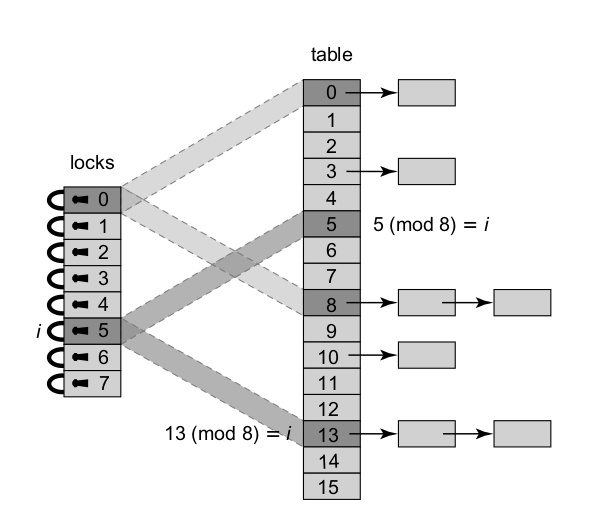
\includegraphics[width=0.7\linewidth]{concurrenciaHT.png}
    \caption{locks in hashtable}
    \label{}
\end{figure}

Para manejar la concurrencia en la tablahash nos basamos en el libro
the art of multiprocessor programming de Maurice Herlihy y Nir Shavit
en el cual, se habla sobre striped hash set y se muestra la figura 1.
Para sincronizar los procesos creamos la misma cantidad de mutexes
que la cantidad de procesadores que tenga la pc que esté corriendo
el programa y particionamos el conjunto de slots del array de listas
de la siguiente manera:

Sea $listaArr$ el array de listas tal que $listArr$ tiene $n$ slots y sea $mutexArr$ el array de mutexes tal que tiene
$m$ elementos.

Definimos los siguientes cojuntos:

$X_0 =\{x\in listArr/x\mod n=0\}$

$X_1 =\{x\in listArr/x \mod n=1\}$

...

$X_m =\{x\in listArr/x \mod n=m\}$ 

Sea $X = \{X_1, X_2, ... , X_m\}$
Notemos que X es una partición de $listArr$. Ahora que
tenemos esta partición, para todo $i\in \mathbb{N}$ tal que
$0 \leq i \leq m$
asignamos $mutexArr[i]$ (elemento
en la posicion cero de mutexArr) a $X_i$.

De esta forma, al tomar el lock $mutexArr[i]$ no
se podrán modificar al mismo tiempo dos
listas que estén en un mismo conjunto $X_i$, pero si
dos listas que estén en diferentes conjuntos.

\subsection{Desalojo}
Para desalojar los elementos creamos una estructura llamada
Evict, la cual es la siguiente.

\begin{lstlisting}[style=CStyle]
struct _Evict {  
  NodeEvict mru;
  NodeEvict lru;
  pthread_mutex_t mutex;  
};
\end{lstlisting}

Esta estructura guarda el elemento más recientemente
usado de la caché (NodeEvict mru), el menos
recientemente usado (NodeEvict lru) y un mutex el cual
se utilizará para modificar o acceder a los datos de
la estructura. Notemos que el tiempo que tengamos el
mutex debe ser mínimo, es decir las modificaciones a 
la estructura evict tienen que ser lo más rápidas
posibles, de otra manera afectará a la concurrencia.

Evict guarda una lista circular de nodos del tipo
NodeEvict, donde cada nodo es de la siguiente forma:
\begin{lstlisting}[style=CStyle]
struct _NodeEvict {
  struct _NodeEvict* next;
  struct _NodeEvict* prev;
  List list;
  unsigned listIdx; //Indice de la lista en la cache
};
\end{lstlisting}

El campo next guarda un puntero al siguiente nodo de
la lista que generalmente es más recientemente usado
que el actual, al menos que el actual sea el mru de
evict, en ese caso next será el lru de evict.

El campo prev guarda un puntero al nodo anterior de la
lista que generalmante es menos recientemente usado
que el actual, al menos que sea el lru de evict, en ese
caso prev será el mru de evict.

El campo list guarda la lista asociado a el nodo de
evict, esto sirve al momento de desalojar al igual
que el campo listIdx.

Hacemos la lista doblemente enlazado para que la
eliminación de nodos se pueda hacer en O(1).

Cuando se necesita eliminar un elemento de evict
se toma el mutex y se intenta eliminar el más recientemente
usado, si no es posible, lo cual podría ocurrir porque
el mutex de el elemento está tomado se intenta eliminar el siguiente elemento más recientemente usado y así sucesivamente,
esto lo hacemos 10 veces y volvemos a empezar, hasta que
consigamos el espacio solicitado o la caché esté vacía.

\end{document}
